\documentclass[11pt, ngerman, fleqn, DIV=15, headinclude, BCOR=2cm]{scrreprt}

\usepackage{../../header}

\usepackage[section]{placeins}

\usepackage{csquotes}

\usepackage{tikz}
\usetikzlibrary{chains}
\usetikzlibrary{shapes.geometric}

\tikzset{device/.style={
                rectangle,
                minimum size=6mm,
                draw=black
            },
            monitor/.style={
                rectangle,
                rounded corners=2mm,
                minimum size=6mm,
                draw=black
            },
        }

\usepackage{pgfplots}
\pgfplotsset{
    compat=1.9,
    width=0.8\linewidth,
    xticklabel style={/pgf/number format/use comma},
    yticklabel style={/pgf/number format/use comma},
}
\usepgfplotslibrary{polar}

\usepgfplotslibrary{external}
\tikzexternalize[mode=list and make]

\DeclareSIUnit{\skt}{SKT}

\usepackage{booktabs}

\hypersetup{
    pdftitle=
}

\subject{Praktikumsprotokoll}
\title{Compton-Effekt}
\subtitle{Versuch P526 -- Universität Bonn}
\author{
    Martin Ueding \\ \small{\href{mailto:mu@martin-ueding.de}{mu@martin-ueding.de}}
    \and
    Lino Lemmer \\
    \small{\href{mailto:l2@uni-bonn.de}{l2@uni-bonn.de}}
}

\date{2014-05-07}

\publishers{Tutor: Roman Schmitz}

\begin{document}

\maketitle

\begin{abstract}
    In diesem Versuch untersuchen wir die Wechselwirkung von
    $\gammaup$-Strahlung mit Materie. Der Schwerpunkt liegt dabei beim
    Compton-Effekt. Zunächst bestimmen wir den Compton-Wirkungsquerschnitt von
    Aluminium, indem wir Targets unterschiedlicher Dicken zwischen Quelle und
    Detektor bringen. Im Anschluss messen wir die Energie des Photopeaks bei
    verschiedenen Streuwinkeln und prüfen so die Klein-Nishina-Gleichung.
\end{abstract}

\tableofcontents

\chapter{Theorie}

Aufgrund der thematischen Überschneidung mit Versuch 525, den vor bereits
durchgeführt haben, übernehmen wir einige Abschnitte aus dem Theorieteil von
\parencite{Ueding/525}.

\section{Wechselwirkung von $\gammaup$-Strahlung mit Materie}
\label{sec:WW}

Trifft $\gammaup$-Strahlung auf Materie, finden abhängig von Photonenergie und
Ordnungszahl des Atoms unterschiedliche Effekte statt. Bei kleinen Energien
($\gamma < 2$) ist der Photoeffekt der stärkste Effekt, bei mittleren Energien
($2 < \gamma < 7$) überwiegt der Comptoneffekt. Bei größeren Energien ist die
Paarerzeugung der Hauptkanal. Die Energien beziehen sich auf Blei als Absorber
und stammen aus \parencite[Abbildung~17.31]{meschede-gerthsen_24}.

\subsection{Photoeffekt}

Als Photoeffekt, auch photoelektrischer oder lichtelektrischer Effekt,
bezeichnet man den Prozess, bei dem ein Photon seine gesamte Energie an ein
Elektron abgibt. Ist diese Energie größer als die Bindungsenergie des
Elektrons, wird dieses aus seiner Bindung gelöst. Die dadurch entstehenden
freien Stellen werden durch höherenergetische Elektronen wieder gefüllt, wobei
sie Photonen emittieren.

Laut \parencite[(2,103)]{Leo/Techniques_Nuclear_Experiments} hängt der
Wirkungsquerschnitt des Photoeffekts ist für nichtrelativistische
Photonenenergien wie folgt mit der Energie $h\nu$ zusammen:
\[
    \sigma \propto Z^5 (h\nu)^{-7/2}.
\]

\subsection{Paarbildung}

Zerfällt ein Photon im Coulombfeld eines Atomkerns in ein
Elektron-Positron-Paar, spricht man von einer Paarbildung. Dies kann nur
stattfinden, wenn die Energie des Photons die Ruheenergie der beiden Teilchen
übersteigt, also $E_\gammaup > 2m_\mathrm{e}c^2$. Zudem findet es bevorzugt bei
hohen Ordnungszahlen statt, da dort die Divergenz des Feldes größer ist.

Der Wirkungsquerschnitt hängt quadratisch von der Ladungszahl ab ($\sigma
\propto Z^2$). Außerdem skaliert er logarithmisch mit der Energie
\parencite[(17.15)]{meschede-gerthsen_24}
\parencite[(2.120)]{Leo/Techniques_Nuclear_Experiments}.

\subsection{Compton-Streuung}

Als Compton-Streuung bezeichnet man die elastische Streuung von Photonen zum
Beispiel an Elektronen. Die dabei vom Photon an das Elektron übertragene
Energie hängt nur vom Winkel ab und ist Maximal bei einem Streuwinkel von $\phi
= \SI{180}\degree$, also bei einer Rückstreuung, und minimal bei $\phi =
\SI{0}\degree$, also wenn das Elektron nur gestreift wird.

\begin{figure}[htbp]
    \centering
    \begin{tikzpicture}
        \draw[->, thick] (-3, 0) -- (0, 0) node[above, midway] {$h\nu$};
        \draw[->, thick] (0, 0) -- (40:3) node[above, midway, sloped] {$h\nu'$};
        \draw[->] (0, 0) -- (-60:2) node[below, midway, sloped] {$T$};
        
        \draw[dashed] (0, 0) -- (4, 0);

        \draw (1.1, 0) arc (0:40:1.1) node[below] {$\phi$};
        \draw (1, 0) arc (0:-60:1) node[above] {$\theta$};
    \end{tikzpicture}
    \caption{%
        Zur Kinematik der Comptonstreuung, nach
        \parencite[Abbildung~2.22]{Leo/Techniques_Nuclear_Experiments}.
    }
    \label{fig:}
\end{figure}

Aus Energie und Impulserhaltung folgt die Beziehung zwischen ein- und
ausgehendem Photon \parencite[(2.106)]{Leo/Techniques_Nuclear_Experiments}:
\[
    h\nu' = \frac{h\nu}{1 + \gamma(1 - \cos(\phi))},
\]
wobei $\gamma := h \nu / m_\text e c^2$ ist. Aus dieser Beziehung, der
Klein-Nishina-Gleichung, kann man
herleiten, dass die Wellenlängendifferenz gegeben ist durch:
\[
    \Deltaup \lambda = \frac{h}{m_\text e c} (1 - \cos(\phi)).
\]
Der Vorfaktor wird auch Comptonwellenlänge genannt.

Werden nun viele Photonen mit einer Energie $E_\nu$ gestreut, wie es in einem
Szintillator der Fall ist, ergibt sich ein charakteristisches Bild. In
Abbildung~\ref{fig:Compton} ist idealisiert die Intensität gegen die an den
Szintillator übertragene Energie dargestellt. Das Compton-Kontinuum entsteht
durch die Streuung mit unterschiedlichen Winkeln, die Compton-Kante wird durch
den maximalen Energieübertrag bei $\phi = \SI{180}{\degree}$ erzeugt. Der
Photopeak, oder auch Full-Energy-Peak bei $E_\nu$ entsteht durch die
vollständige Deponierung der Photonenergie im Szintillator, beispielsweise
durch den Photoeffekt. Die Restenergie des zurück gestreuten Photons ist genau
die Differenz von $E_\nu$ und der Energie an der Compton-Kante.

\begin{figure}[htbp]
    \centering
    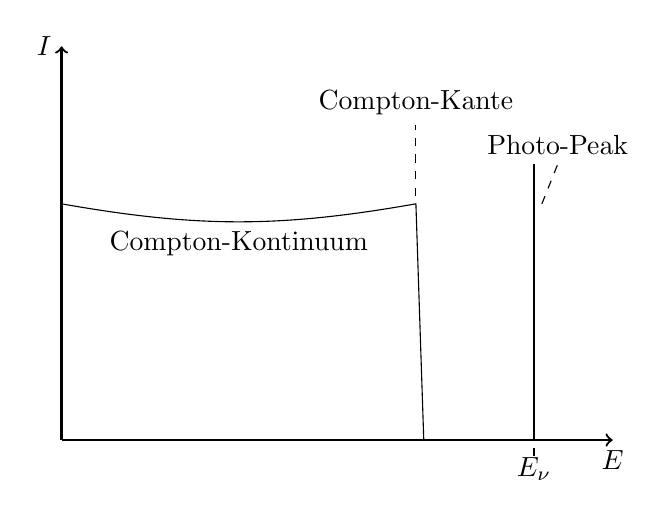
\begin{tikzpicture}
        \draw[thick,->]
        (0,0) -- (0,5) node[left] {$I$}
        ;
        \draw[thick,->]
        (0,0) -- (7,0) node[below] {$E$}
        ;
        \draw
        (6,0) -- (6,3.5)
        ;
        \draw
        (6,-.2) -- (6,-.1) node[below] {$E_\nu$}
        ;
        \draw[bend right=10]
        (0,3) to node[below] {Compton-Kontinuum} (4.5,3) -- (4.6,0)
        ;
        \draw[dashed]
        (4.5,3.1) -- (4.5,4) node[above] {Compton-Kante}
        ;
        \draw[dashed]
        (6.1,3) -- (6.3,3.5) node[above] {Photo-Peak}
        ;
    \end{tikzpicture}
    \caption{%
        Idealisiertes Spektrum der bei Einstrahlung von monochromatischer
        $\gammaup$-Strahlung an den Szintillator übertragenen Energie
    }
    \label{fig:Compton}
\end{figure}

\subsubsection{Differentieller Wirkungsquerschnitt}

Die Klein-Nishina Formel wurde aus der QFT hergeleitet und ist
\parencite[(2.107)]{Leo/Techniques_Nuclear_Experiments}
\[
    \dod\sigma\Omega =
    \frac{r_\text e^2}2 \frac1{\del{1 + \gamma(1 - \cos(\theta))}^2}
    \del{
        1 + \cos(\theta)^2 + \frac{\gamma^2(1 - \cos(\theta)^2)}{1 + \gamma(1 -
        \cos(\theta))}
    }.
\]
Sie beschreibt den differentiellen Wirkungsquerschnitt der Compton-Streuuung in
Abhängigkeit der Energie und des
Polarwinkels $\theta$.

\subsubsection{Totaler Stoßwirkungsquerschnitt}

Durch Integration des differentiellen Wirkungsquerschnitts nach dem Raumwinkel
erhält man den totalen Wirkungsquerschnitt. Dieser ist in
\parencite[(2.107)]{Leo/Techniques_Nuclear_Experiments} gegeben als
\[
    \sigma = 2 \piup r_\text e^2 \del{
        \frac{1+\gamma}{\gamma^2} \del{
            \frac{2(1+\gamma)}{1+2\gamma} - \frac1\gamma \ln(1+2\gamma)
        }
        + \frac1{2\gamma} \ln(1+2\gamma) - \frac{1+3\gamma}{(1+2\gamma)^2}
    }.
\]

\subsubsection{Abhängigkeit des Wirkungsquerschnitts von $E_\nu$}

Mit $s := T / h \nu$ lässt sich aus der Klein-Nishina Formel das
Energiespektrum herleiten
\parencite[(2.113)]{Leo/Techniques_Nuclear_Experiments}:
\[
    \dod\sigma T =
    \frac{\piup r_\text e^2}{m_\text e c^2 \gamma^2} \del{
        2 + \frac{s^2}{\gamma^2(1 - s)^2} + \frac{s}{1-s} \del{
            s - \frac2\gamma
        }
    }
\]

Im Fall von $\theta = \piup$ wird der meiste Impuls und Energie auf das
Elektron übertragen. Diese Maximalenergie zeigt sich im Spektrum als
„Comptonkante“ und ist gegeben durch
\parencite[(2.114)]{Leo/Techniques_Nuclear_Experiments}
\[
    T_\text{max} = h \nu \frac{2\gamma}{1+2\gamma}.
\]


\subsection{Linearpolarisation von $\boldsymbol\gammaup$-Quanten}

% TODO

\subsection{Abschwächung von $\boldsymbol\gammaup$-Strahlung in Materie}

Wechselwirken Photonen mit Materie, so wird in der Regel ihre
Ausbreitungsrichtung geändert. Dies bewirkt, dass sie danach nicht mehr im
Strahl sind. Im Gegensatz zu Teilchen, die auf einer geraden Strecke
kontinuierlich Energie an das Medium abgeben können, reduziert sich bei
Photonen nur deren Rate, nicht jedoch die Energie eines einzelnen Photons.

Ist die Anzahldichte der Streuzentren $n$, so ist $n \dif x$ eine Flächendichte
für eine Schicht der Dicke $\dif x$. Jedes Streuzentrum habe den
Wirkungsquerschnitt $\sigma$. Somit ist ein Anteil $n \dif x \sigma$ für die
Transmission versperrt. Die Intensität nimmt also um diesen Anteil in der
dünnen Schicht ab:
\[
    \dif I = - n \dif x \sigma I.
\]

Diese Differentialgleichung kann durch Teilen durch $\dif x$ und Integration
gelöst werden:
\[
    I(x) = I_0 \exp(- n \sigma x).
\]
Dies ist die Formel von Lambert-Beer. $n \sigma$ ist der \emph{totale
Abschwächungskoeffizient}.

\subsection{Klein-Nishina-Plot}

Im Klein-Nishina-Plot wird der differentielle Wirkungsquerschnitt gegen den
Winkel aufgetragen, jedoch in einem Polardiagramm. Theoretische Graphen sind in
Abbildung~\ref{fig:nishina-theo} dargestellt.

\begin{figure}[htbp]
    \centering
    \begin{tikzpicture}
        \begin{polaraxis}[
                width=0.9\linewidth,
                xmin=0,
                xmax=180,
                legend entries={
                    $\gamma=\num{0.01}$,
                    $\gamma=\num{0.1}$,
                    $\gamma=\num{1}$,
                    $\gamma=\num{10}$,
                }
            ]
            \addplot[Red] table {plot_klein_nishina_1.txt};
            \addplot[Green] table {plot_klein_nishina_2.txt};
            \addplot[Blue] table {plot_klein_nishina_3.txt};
            \addplot[Purple] table {plot_klein_nishina_4.txt};
        \end{polaraxis}
    \end{tikzpicture}
    \caption{%
        Klein-Nishina-Plot: Differentieller Wirkungsquerschnitt
        $\od\sigma\Omega$ in Abhängigkeit des Polarwinkels $\phi$.
    }
    \label{fig:nishina-theo}
\end{figure}

\subsection{Thomsonstreuung}

Die Thomsonstreuung ist der niederenergetische Grenzfall der Comptonstreuung.
In diesem Fall wird keine Energie an das Elektron übertragen. Dadurch sind
diese Effekte nur dafür verantwortlich, dass die Ausbreitungsrichtung der
Photonen geändert wird. Ist die Photonenenergie deutlich kleiner als die
Elektronenmasse, so vereinfacht sich die Klein-Nishina-Formel zu
\parencite[(2.115)]{Leo/Techniques_Nuclear_Experiments}
\[
    \sigma = \frac{8\piup}3 r_\text e^2.
\]

\subsection{Rückstreu- und Escape-Peak}

Wird ein Photon, nachdem es durch den Compton-Effekt zurückgeworfen wurde, ein
weiteres Mal um $\phi = \SI{180}{\degree}$ gestreut, oder in einem
gegenüberliegenden Szintillator detektiert, entsteht ein weiterer Peak, der
eine Spektrallinie vortäuscht. Dies ist der Rückstreu-Peak. Die Energie dieses
Peaks ist daher identisch mit der Restenergie des Photons.

Kommt es zur Paarbildung, wird nur dann die volle Energie im Szintillator
deponiert, wenn das entstehende Positron auf ein Elektron trifft, unter Abgabe
zweier \SI{511}{\kilo\electronvolt}-Photonen annihilliert und beide
entstehenden Photonen durch andere Effekte ihre Energie an den Szintillator
abgeben. Verlässt eines der Photonen oder sogar beide den Szintillator, ohne
Energie abzugeben, entsteht eine weitere scheinbare Spektrallinie, der Single-
bzw. Double-Escape-Peak, bei einer Energie von
$E_\nu-\SI{511}{\kilo\electronvolt}$ bzw. $E_\nu-\SI{1022}{\kilo\electronvolt}$.

% TODO Form des Spektrums.

% TODO Peak to Total Verhältnis.

\section{Instrumente}

\subsection{Szintillator}

Zur Detektion von $\gammaup$-Quanten verwendet man einen Kristall, zum Beispiel
Natriumiodid. Trifft nun ein $\gammaup$ auf ein Elektron, wird es durch die
Effekte aus \ref{sec:WW} angeregt. Bei einer Abregung über Zwischenniveaus
werden Photonen niedrigerer Energie abgegeben, welche von einem
Photomultiplier eingefangen werden können. Eine andere Möglichkeit ist der
Stoß mit anderen Elektronen, wodurch zwei Elektronen mit geringerer Energie
entstehen. Die Intensität des Lichtblitzes ist dabei proportional zur Energie
des ursprünglichen $\gammaup$-Quants.

\subsubsection{Energieauflösung}

Durch verschiedene Effekte im Szintillator, die durch die endliche Temperatur
verursacht werden, ist die Energieauflösung $E/\Deltaup E$ beschränkt. Im
Versuch 525 haben wir eine Auflösung in der Größenordnung von 5 gehabt.

\subsubsection{Totzeit}

Die eintreffenden Photonen erzeugen Teilen- und Antiteilchenschauer im
Szintillator, die eine gewisse Lebenszeit haben. Trifft in dieser Zeit ein
zweites Photon ein, so kann es zu Überschneidungen kommen und die Signale nicht
mehr getrennt werden. Daher braucht der Szintillator eine gewisse Zeit, bis
alle erzeugten Teilchen wieder gebunden sind. Diese Zeit wird Totzeit genannt.

\subsubsection{Selbsttransparenz}

Die Dotierung im Kristall sorgt dafür, dass es Übergänge mit weniger als der
Bindungsenergie gibt. Rekombiniert ein Elektron in ein derartiges Loch, so ist
die Energie des frei werdenden Photons kleiner als die normale
Ionisationsenergie. Dadurch kann es keine weiteren Elektronen auslösen, der
Kristall ist für diese Photonen transparent.

\subsection{Photomultiplier (PM)}

Will man ein schwaches optisches Signal in eine messbares elektrisches Signal
umwandeln, benötigt man einen Photomultiplier. Ein möglicher Aufbau ist in
Abbildung~\ref{fig:PM} zu sehen. Zwischen Photokathode und Anode liegt eine
Spannung an, die von Dynode zu Dynode abfällt.

Trifft ein Photon auf die Photokathode, löst es, wenn seine Energie die
Austrittsarbeit übersteigt, ein Elektron aus dieser heraus. Durch die angelegte
Spannung wird das Elektron beschleunigt und zum Beispiel durch ein Elektrisches
Feld so abgelenkt, dass es auf die erste Dynode trifft. Hier löst es weitere
Elektronen aus, die zur nächsten Dynode beschleunigt werden. Der Prozess geht
so weiter, bis zum Schluss die Lawinenelektronen auf die Anode treffen und dort
ein messbares elektronisches Signal ergeben.

Da die Anzahl der ausgelösten Elektronen proportional zur Intensität der
eintreffenden Strahlung ist, und da der Photomultiplier linear verstärkt, ist
das Ausgangssignal proportional zur einfallenden Intensität. Wird ein
Szintillatorsignal verstärkt, ist die Amplitude also proportional zur Energie
der $\gammaup$-Strahlung.

An der Anode liegt meistens Sättigung vor. Dies sorgt dafür, dass die Amplitude
des Signals keine Aussage mehr über die Energie machen kann aber durch eine
Anstiegszeit von wenigen \si{\nano\second} eine hohe Zeitgenauigkeit erreicht
wird. Wegen des schnellen Anstiegs wird das Ausgangssignal daher auch
\emph{Fast}-Signal genannt.

Greift man das Signal an einer Dynode, an der noch keine Sättigung herrscht ab,
ist eine Aussage über die Energie des verursachenden Photons möglich. Die
Anstiegszeit ist jedoch deutlich größer. Daher heißt dieses Signal auch
\emph{Slow}-Signal.

\begin{figure}[htbp]
    \centering
    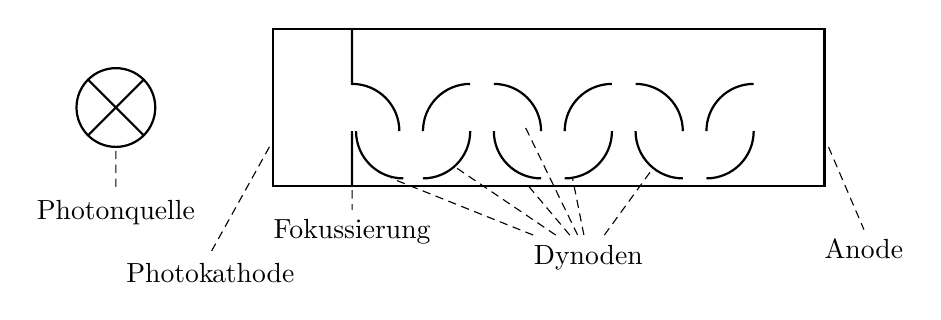
\begin{tikzpicture}
        % Röhre
        \draw[thick] (2,-1) rectangle (9,1);
        % Photonquelle
        \draw[thick]
        (0,0) circle (.5)
        (225:.5) -- (45:.5)
        (135:.5) -- (-45:.5)
        ;
        % Photokathode und Anode
        \draw[thick]
        (2,1) -- (2,-1)
        (9,1) -- (9,-1)
        ;
        % Dynoden
        \draw[thick]
        (3,-.3) -- (3,-1)
        (3,1) -- (3,.3) arc (90:0:.6cm)
        (3.05,-.3) arc (180:270:.6cm)
        (3.9,-.9) arc (270:360:.6cm)
        (3.9,-.3) arc (180:90:.6cm)
        (4.8,.3) arc (90:0:.6cm)
        (4.8,-.3) arc (180:270:.6cm)
        (5.7,-.9) arc (270:360:.6cm)
        (5.7,-.3) arc (180:90:.6cm)
        (6.6,.3) arc (90:0:.6cm)
        (6.6,-.3) arc (180:270:.6cm)
        (7.5,-.9) arc (270:360:.6cm)
        (7.5,-.3) arc (180:90:.6cm)
        ;
        % Beschriftungen PQ, PK, A und Fokussierung
        \draw[densely dashed]
        (0,-.55) -- (0,-1.05) node[below] {Photonquelle}
        (1.95,-.5) -- (1.2,-1.85) node[below] {Photokathode}
        (3,-1.05) -- (3,-1.3) node[below] {Fokussierung}
        (9.05,-.5) -- (9.5,-1.55) node[below] {Anode}
        ;
        % Beschriftung Dynoden
        \node (D) at (6,-1.9) {Dynoden};
        \draw[densely dashed]
        (D) -- (3.5,-.9)
        (D) -- (4.3,-.75)
        (D) -- (5.2,-.95)
        (D) -- (5.2,-.25)
        (D) -- (5.8,-.9)
        (D) -- (6.8,-.8)
        ;
    \end{tikzpicture}
    \caption{%
        Möglicher Aufbau eines Photomultipliers
    }
    \label{fig:PM}
\end{figure}

\subsection{Vielkanalanalysator (MCA)}

Der Vielkanalanalysator (engl. \emph{multi channel analyzer}) sortiert
einkommende Signale nach Amplitude. Trifft ein Signal mit einer bestimmten
Amplitude ein, setzt er einen Zähler in einem bestimmten Kanal hoch. Dadurch
zählt der MCA wie häufig die verschiedenen Amplituden auftauchen. Es entsteht
eine Art Histogramm.

\section{Zerfallsschemata}

\begin{figure}[htbp]
    \centering
    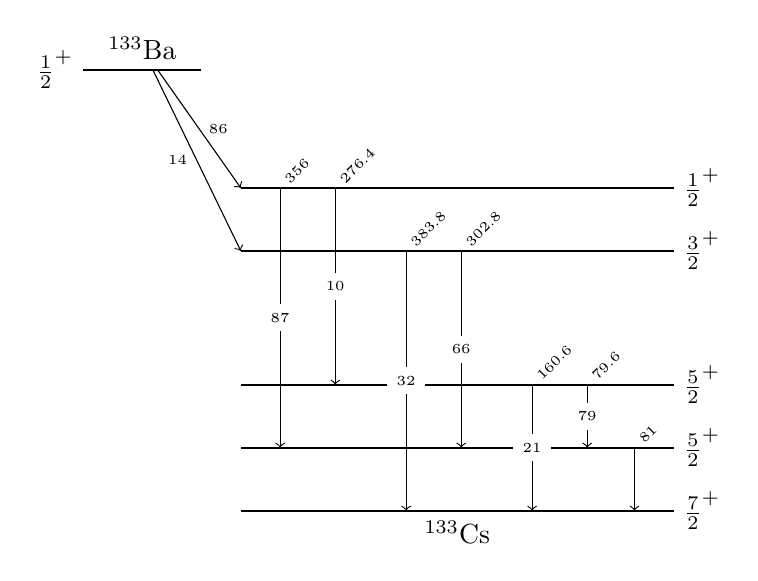
\begin{tikzpicture}
        \draw[thick]
        (-.5,5) node[left]{$\frac12^+$} -- node[above] (Ba) {${}^{133}$Ba} (1,5)
        (1.5,3.5) coordinate (EC1) -- (7,3.5) node[right] {$\frac12^+$}
        (1.5,2.7) coordinate (EC2) -- (7,2.7) node[right] {$\frac32^+$}
        (1.5,1.0)  -- (7,1.0) node[right] {$\frac52^+$}
        (1.5,0.2)  -- (7,0.2) node[right] {$\frac52^+$}
        (1.5,-0.6) -- node[below] {${}^{133}$Cs} (7,-0.6) node[right] {$\frac72^+$}
        ;
        \draw[->]
        (Ba) -- node[right]{\tiny{\SI{86}{\percent}}} (EC1)
        ;
        \draw[->]
        (Ba) -- node[left]{\tiny{\SI{14}{\percent}}} (EC2)
        ;
        % Linien
        \draw[->]
        (2,3.5) node[right, rotate=45]
        {\tiny{\SI{356}{\kilo\electronvolt}}} -- node[midway,
        fill=white] {\tiny{\SI{87}{\percent}}} (2,.2)
        ;
        \draw[->]
        (2.7,3.5) node[right, rotate=45]
        {\tiny{\SI{276.4}{\kilo\electronvolt}}} -- node[midway,
        fill=white] {\tiny{\SI{10}{\percent}}} (2.7,1.)
        ;
        \draw[->]
        (3.6,2.7) node[right, rotate=45]
        {\tiny{\SI{383.8}{\kilo\electronvolt}}} -- node[midway,
        fill=white] {\tiny{\SI{32}{\percent}}} (3.6,-.6)
        ;
        \draw[->]
        (4.3,2.7) node[right, rotate=45]
        {\tiny{\SI{302.8}{\kilo\electronvolt}}} -- node[midway,
        fill=white] {\tiny{\SI{66}{\percent}}} (4.3,.2)
        ;
        \draw[->]
        (5.2,1.0) node[right, rotate=45]
        {\tiny{\SI{160.6}{\kilo\electronvolt}}} -- node[midway,
        fill=white] {\tiny{\SI{21}{\percent}}} (5.2,-.6)
        ;
        \draw[->]
        (5.9,1.0) node[right, rotate=45]
        {\tiny{\SI{79.6}{\kilo\electronvolt}}} -- node[midway,
        fill=white] {\tiny{\SI{79}{\percent}}} (5.9,.2)
        ;
        \draw[->]
        (6.5,.2) node[right, rotate=45]
        {\tiny{\SI{81}{\kilo\electronvolt}}} -- (6.5,-.6)
        ;
    \end{tikzpicture}
    \caption{%
        Zerfallsschema von ${}^{133}$Ba. Übernommen aus \parencite{Ueding/525}.
    }
    \label{fig:Ba-Zerfall}
\end{figure}

% TODO Zerfallsschema 137Cs.

\chapter{Durchführung}

\section{Vorbereitung}

% 01_Untergrund001.txt

\section{Totaler Stoßwirkungsquerschnitt}

\section{Energiekalibrierung des Spektrometers}

\section{Messung der Streuspektren}

\chapter{Auswertung}

\section{Abschwächungskoeffizient}

Aus den Messdaten für den Wirkungsquerschnitt wählen wir das letzte Maximum
aus. An diese Auswahl passen wir die Normalverteilung
\begin{equation}
    \frac{a}{\sqrt{2\piup} \sigma} \exp\del{\frac{(x-\mu)^2}{2\sigma^2}}
    \label{eq:gausskurve}
\end{equation}
an, deren Integral einfach nur $a$ ist. Die Daten und Anpassungskurven sind in
Abbildung~\ref{fig:amplituden} dargestellt. In Tabelle~\ref{tab:amplituden}
sind die Anpassungsparameter zusammengestellt.

\begin{figure}[htbp]
    \centering
    \begin{tikzpicture}
        \begin{axis}[
                width=\linewidth,
                height=0.6\linewidth,
                xlabel=Kanal,
                ylabel=Ereignisse,
                grid=major,
            ]
            \addplot[gray] table {plot-decay-data-00mm.txt};
            \addplot[black] table {plot-decay-used-00mm.txt};

            \addplot[gray] table {plot-decay-data-01mm.txt};
            \addplot[black] table {plot-decay-used-01mm.txt};

            \addplot[gray] table {plot-decay-data-05mm.txt};
            \addplot[black] table {plot-decay-used-05mm.txt};

            \addplot[gray] table {plot-decay-data-10mm.txt};
            \addplot[black] table {plot-decay-used-10mm.txt};

            \addplot[gray] table {plot-decay-data-20mm.txt};
            \addplot[black] table {plot-decay-used-20mm.txt};

            \addplot[gray] table {plot-decay-data-50mm.txt};
            \addplot[black] table {plot-decay-used-50mm.txt};

            \addplot[red, thick] table {plot-decay-fit-00mm.txt};
            \addplot[red, thick] table {plot-decay-fit-01mm.txt};
            \addplot[red, thick] table {plot-decay-fit-05mm.txt};
            \addplot[red, thick] table {plot-decay-fit-10mm.txt};
            \addplot[red, thick] table {plot-decay-fit-20mm.txt};
            \addplot[red, thick] table {plot-decay-fit-50mm.txt};

        \end{axis}
    \end{tikzpicture}
    \caption{%
        Spektrum der eingebauten Quelle ohne Absorber und mit
        \SIlist{1;5;10;20;50}{\milli\meter} Aluminium. An die schwarz
        markierten Punkte wurden Normalverteilungen angepasst, diese sind in
        rot darüber gezeigt.
    }
    \label{fig:amplituden}
\end{figure}

Nach dem Lambert-Beer-Gesetz ist eine exponentielle Abschwächung der
Strahlungsleistung (hier repräsentiert durch das Integral) zu erwarten. Daher
passen wir an die Daten eine Zerfallsfunktion,
\[
    I(x) = I_0 \exp(- a x),
\]
an. Den letzen Punkt haben wir bei der Anpassung ausgelassen, da er sehr weit
von der Kurve entfernt liegt. Das Aluminiumstück, das für die die letzte
Messung benutzt haben, war sehr schmal. Dadurch ist es zum einen schwer
gewesen, es wirklich parallel zum Strahlengang auszurichten, außerdem könnte
Strahlung auch neben dem Stück passiert und in den Detektor gelangt sein. Der
Wirkungsquerschnitt ist demnach nicht so gering, wie bei dieser Dicke zu
erwarten wäre.

Da $a = \SI{<< alu_a >>}{\per\milli\meter} = n
\sigma$\footnote{\erklaerungFehlerNotation} ist, erhalten wir
mit der Dichte $\rho = \SI{<< alu_dichte >>}{\gram\per\cubic\milli\meter}$ und
der Atommasse $m = \SI{<< alu_amu >>}{\atomicmassunit}$ von Aluminium, sowie
der Anzahldichte $n = \rho N_\text A / m = \SI{<< alu_n
>>}{\per\cubic\milli\meter}$ einen Wirkungsquerschnitt von $\sigma = \SI{<<
alu_sigma >>}{\barn}$. Dies liegt in der angekündigten Größenordnung.

\begin{table}[htbp]
    \centering
    \begin{tabular}{SSSS}
        {Dicke / \si{\milli\meter}} &
        {Integral / Kanal} &
        {$\mu$ / Kanal} &
        {$\sigma$ / Kanal} \\
        \midrule
        %< for row in decay_table: ->%
        << ' & '.join(row) >> \\
        %< endfor ->%
    \end{tabular}
    \caption{%
        Anpassungsparameter für die verschiedenen Dicken der
        Absorbermaterialien.
    }
    \label{tab:amplituden}
\end{table}

\begin{figure}[htbp]
    \centering
    \begin{tikzpicture}
        \begin{axis}[
                width=\linewidth,
                height=0.6\linewidth,
                xlabel=Kanal,
                ylabel=Integral,
                grid=major,
            ]
            \addplot[
                black,
                mark=|,
                only marks,
                error bars/.cd,
                y dir=both, y explicit,
            ]
            table[y error index=2] {plot-decay-data.txt};
            \addplot[red] table {plot-decay-fit.txt};
        \end{axis}
    \end{tikzpicture}
    \caption{%
        Maximale Amplitude gegen Absorberdicke. Die Messpunkte stammen aus den
        Anpassungen der vorherigen Abbildung. Der letze Punkt wurde aus der
        Anpassung ausgeschlossen. Die Fehlerbalken sind in der Abbildung,
        jedoch sind diese extrem klein.
    }
    \label{fig:decay}
\end{figure}

Wir haben zusätzlich die Spektren mit einen Gaußkern gefaltet ($\sigma =
\num{<< extinction_gauss_sigma >>}$\,Kanäle), um diese zu glätten. Danach haben
wir die Spektren durch das ohne Absorber geteilt, um ein Auslöschungsverhältnis
zu erhalten. Diese normalisierten Spektren haben wir in
Abbildung~\ref{fig:extinktion} dargestellt.

\begin{figure}[htbp]
    \centering
    \begin{tikzpicture}
        \begin{axis}[
                width=\linewidth,
                height=0.6\linewidth,
                xlabel=Kanal,
                ylabel=Extinktionsfaktor,
                grid=major,
            ]
            \addplot[black] table {plot-ratio-00mm.txt};
            \addplot[black] table {plot-ratio-01mm.txt};
            \addplot[black] table {plot-ratio-05mm.txt};
            \addplot[black] table {plot-ratio-10mm.txt};
            \addplot[black] table {plot-ratio-20mm.txt};
            \addplot[black] table {plot-ratio-50mm.txt};
        \end{axis}
    \end{tikzpicture}
    \caption{%
        Extinktionsfaktoren nach Glättung, ohne Absorber (per Definition
        konstant 1) sowie mit \SIlist{1;5;10;20;50}{\milli\meter} Aluminium
        zwischen eingebauter Quelle und Detektor.
    }
    \label{fig:extinktion}
\end{figure}

\section{Energieeichung}

Zur Energieeichung betrachten wir zunächst den
\SI{662}{\kilo\electronvolt}-Übergang im ${}^{137}$Ba. An diesen passen wir
eine Gaußkurve wie in Gleichung~\eqref{eq:gausskurve} beschrieben an. Die Daten
sind samt Anpassung in Abbildung~\ref{fig:eichung_137Ba} dargestellt.

\begin{figure}[htbp]
    \centering
    \begin{tikzpicture}
        \begin{axis}[
                width=\linewidth,
                height=0.6\linewidth,
                xlabel=Kanal,
                ylabel=Ereignisse,
                grid=major,
            ]
            \addplot[black] table[skip first n=117] {../Daten/01_Untergrund001.txt};
            \addplot[red, thick] table {fit_peak_662.txt};
        \end{axis}
    \end{tikzpicture}
    \caption{%
        Energiespektrum von ${}^{137}$Ba. Zu erkennen ist der Full-Energy-Peak
        im Bereich von Kanal 3000 bis 3700, das Compton-Kontinuum etwa bis
        Kanal 2200 und der Rückstreu-Peak circa bei Kanal 1000.
    }
    \label{fig:eichung_137Ba}
\end{figure}
 
Genauso gehen wir beim Spektrum von ${}^{133}$Cs vor. Hier passen wir
Gaußkurven an die \SI{31}{\kilo\electronvolt}-Röntgenlinie und die
\SI{81}{\kilo\electronvolt}- und
\SI{356}{\kilo\electronvolt}-$\gammaup$-Linien an. Da letztere und die weniger
ausgeprägte \SI{302}{\kilo\electronvolt}-Linie nicht aufgelöst werden können,
passen wir hier eine Überlagerung zweier Gaußkurven an, wählen für die
Energieeichung aber nur die höherenergetische Linie aus. Die Daten sind
einschließlich der Anpassungskurven in Abbildung~\ref{fig:eichung_133Cs} zu
sehen. 

\begin{figure}[htbp]
    \centering
    \begin{tikzpicture}
        \begin{axis}[
                width=\linewidth,
                height=0.6\linewidth,
                xlabel=Kanal,
                ylabel=Ereignisse,
                grid=major,
            ]
            \addplot[black] table[skip first n=83] {../Daten/Spektrum_Ba001.txt};
            \addplot[red, thick] table {fit_peak_31.txt};
            \addplot[red, thick] table {fit_peak_81.txt};
            \addplot[red, thick] table {fit_peak_356.txt};
        \end{axis}
    \end{tikzpicture}
    \caption{%
        Energiespektrum von ${}^{133}$Cs. Zu erkennen ist die
        \SI{31}{\kilo\electronvolt}-Röntgenlinie und die
        \SI{81}{\kilo\electronvolt}- und
        \SI{356}{\kilo\electronvolt}-$\gammaup$-Linien.
    }
    \label{fig:eichung_133Cs}
\end{figure}

Aus den Anpassungen erhalten wir die in Tabelle~\ref{tab:energieeichung}
dargestellten Zuordnungen.

\begin{table}[htbp]
    \centering
    \begin{tabular}{SSS}
        {$\mu$ / Kanal} & {$\sigma$/ Kanal} & {Energie /
    \si{\kilo\electronvolt}}\\
    \midrule
    %< for a, b, c in data_energieeichung: ->%
    << a >> & << b >> & << c >> \\
    %< endfor ->%
    \end{tabular}
    \caption{%
        Schwerpunkte und Breiten der Anpassungen an die jeweiligen Linien.
    }
    \label{tab:energieeichung}
\end{table}

Um damit den Kanal in eine Energie umrechnen zu können, passen wir an diese
Daten eine Gerade an. Dies ist in Abbildung~\ref{fig:energieeichung} zu sehen.
Für die Anpassung ergibt sich
\[
    E = \SI{<< fit_energieeichung_steigung >>}{\kilo\electronvolt}\cdot \text{Kanal}
    + \del{\SI{<< fit_energieeichung_offset >>}{\kilo\electronvolt}}.
\]

\begin{figure}
    \centering
    \begin{tikzpicture}
        \begin{axis}[
                width=\linewidth,
                height=0.6\linewidth,
                xlabel=Kanal,
                ylabel=Energie / \si{\kilo\electronvolt},
                no markers,
                xtick={0,500,...,3500},
                grid=major,
            ]
            \addplot[scatter, only marks,
                error bars/.cd,
                x dir=both, x explicit,
            ]
            table[x error index=2] {data_energieeichung.txt};
            \addplot[red] table {fit_energieeichung.txt};
        \end{axis}
    \end{tikzpicture}
    \caption{%
        Geradenanpassung zur Energieeichung
    }
    \label{fig:energieeichung}
\end{figure}

\FloatBarrier
\section{Messung der Streuspektren}

Nun wird der Detektor auf in einem Winkel von \SI{40}{\degree} zur Strahlachse
aufgestellt. Als Target wählen wir einen ca. \SI{20}{\milli\meter} starken
Plexiglas-Zylinder. Wir messen nun das Spektrum
jeweils \SI{300}{\second} lang in \SI{5}{\degree}-Schritten bis zu einem Winkel
von \SI{120}{\degree} durch und führen für jede Messung noch eine
Untergrundmessung mit gleicher Messdauer durch. Die korrigierten Spektren sind
in den Abbildungen~\ref{fig:spek_40deg} bis \ref{fig:spek_120deg} zu sehen.

%< for angle in range(40, 121, 5): >%
\begin{figure}
    \centering
    \begin{tikzpicture}
        \begin{axis}[
                width=\linewidth,
                height=0.6\linewidth,
                xlabel=Energie / \si{\kilo\electronvolt},
                ylabel=Ereignisse,
                grid=major,
            ]
            \addplot[
                error bars/.cd,
                x dir=both, x explicit,
                y dir=both, y explicit,
            ]
            table {spektrum_<< angle >>deg_korr.txt};
            \addplot[red, thick] table {fit_<< angle >>deg.txt};
        \end{axis}
    \end{tikzpicture}
    \caption{%
        Spektrum bei \SI{<< angle >>}{\degree}
    }
    \label{fig:spek_<< angle >>deg}
\end{figure}
%< endfor >%

\clearpage

Die aus den Anpassungen erhaltenen Schwerpunktsenergien werden nun gegen
\[
    \frac1{1+\frac{E_\gammaup}{m_\text{e}c^2}\del{1-\cos\phi}}
\]
aufgetragen, wobei $E_\gammaup$ die ursprüngliche Energie des Übergangs ist. Nach der
Klein-Nishina-Formel sollte dies eine Gerade mit Steigung $E_\gammaup$ ergeben.
Die graphische Darstellen einschließlich der idealen Gerade ist in
Abbildung~\ref{fig:E_winkelabhaengigkeit} zu sehen. In
Abbildung~\ref{fig:nishina-ex} ist die gleiche Abhängigkeit nicht linearisiert
in einem Polardiagramm dargestellt.

\begin{figure}[htbp]
    \centering
    \begin{tikzpicture}
        \begin{axis}[
                width=\linewidth,
                height=0.6\linewidth,
                xlabel=$\del{1+\frac{E_\gammaup}{m_\text{e}c^2}\del{1-\cos\phi}}^{-1}$,
                ylabel=Energie / \si{\kilo\electronvolt},
                grid=major,
                no markers,
            ]
            \addplot[
                scatter, only marks,
                error bars/.cd,
                x dir=both, x explicit,
                y dir=both, y explicit,
            ]
            table[x error index=2, y error index=3] {E_winkelabhaengigkeit.txt};
            \addplot[black] table {E_winkelabhaengigkeit_ideal.txt};
        \end{axis}
    \end{tikzpicture}
    \caption{%
        Winkelabhängigkeit der Photonenergie nach Compton-Streuung. Die
        Gerade beschreibt die mit der Klein-Nishina-Formel vorhergesagte
        Abhängigkeit.
    }
    \label{fig:E_winkelabhaengigkeit}
\end{figure}

\begin{figure}[htbp]
    \centering
    \begin{tikzpicture}
        \begin{polaraxis}[
                width=0.9\linewidth,
                xmin=0,
                xmax=180,
                xlabel={$\phi / \si\degree$},
                ylabel=Energie / \si{\kilo\electronvolt},
            ]
            \addplot[black, only marks] table {E_winkelabhaengigkeit_polar.txt};
        \end{polaraxis}
    \end{tikzpicture}
    \caption{%
        Winkelabhängigkeit der Photonenergie nach Compton-Streuung als
        Polardiagramm.
    }
    \label{fig:nishina-ex}
\end{figure}


\chapter{Ergebnis}

% TODO Ergebnis.

\end{document}

% vim: spell spelllang=de tw=79
